\documentclass[11pt, a4paper]{article}

% ----- Packages -----
\usepackage[utf8]{inputenc}
\usepackage{amsmath, amssymb, amsthm, mathtools}
\usepackage{geometry}
\geometry{top=1in, bottom=1in, left=1in, right=1in}
\usepackage{float}
\usepackage{tikz}
\usepackage{xcolor}
\usepackage{booktabs}
\usepackage{graphicx}
\usepackage{fancyhdr}
\usepackage{lastpage}
\usepackage[colorlinks=true, linkcolor=blue, citecolor=blue, urlcolor=blue]{hyperref}
\usepackage[capitalise, noabbrev]{cleveref}
\usetikzlibrary{arrows.meta, positioning, decorations.pathmorphing, patterns, calc}

% ----- Fancy Headers/Footers -----
\pagestyle{fancy}
\fancyhf{}
\fancyhead[L]{\small CE 512 --- Finite Element Method}
\fancyhead[R]{\small Homework 1}
\fancyfoot[C]{\small Page \thepage\ of \pageref{LastPage}}
\renewcommand{\headrulewidth}{0.4pt}
\renewcommand{\footrulewidth}{0.4pt}

% ----- TikZ Styles -----
\tikzset{
    feNode/.style={circle, draw=black, fill=white, thick, inner sep=0pt, minimum size=1.8mm},
    dimLine/.style={|<->|, >=Latex, thick}
}

\begin{document}

% ----- Title Page -----
\begin{titlepage}
\thispagestyle{empty}
\begin{center}
    \vspace*{1cm}
    
\includegraphics[width=0.45\textwidth]{iyte_logo eng.pdf}\\[1.5cm]
    {\LARGE \textbf{Homework 1 --- Solutions}}\\[0.8cm]
    {\Large \textbf{CE 512 Finite Element Method}}\\[0.4cm]
    {\Large 2026 Spring}\\[2.5cm]
    {\large \textbf{Muhammet Ya\u{g}c\i o\u{g}lu}}\\[0.3cm]
    {\large Student No: 290204042}\\[2cm]
    {\large February 26, 2026}
    \vfill
    {\normalsize \textit{\. Izmir Institute of Technology}\\Department of Civil Engineering}
\end{center}
\end{titlepage}

% ----- Table of Contents, Figures, Tables -----
\tableofcontents
\listoffigures
\listoftables
\newpage

% ======================================================================
%  1. INTRODUCTION
% ======================================================================
\section{Introduction}

This report solves three 1D element problems: axial truss, cold conduction, and resistive wire.  They share the same element geometry and shape functions.  Only the field variable, material law, and sign convention differ.  Indices $\alpha,\beta\in\{i,j\}$ label the nodes; no summation is implied.

% ======================================================================
%  2. GENERAL DEFINITIONS
% ======================================================================
\section{Element Geometry, Shape Functions, and General Definitions}

\subsection{Element domain, boundary, and interpolation}\label{sec:geom}

Let $(e)$ denote the oriented 1--simplex with the material coordinate $x\in[0,L]$, node~$i$ at $x=0$, node~$j$ at $x=L$, and outward unit normals $n_i=-1$ at $x=0$, $n_j=+1$ at $x=L$.

\begin{figure}[H]
\centering
\resizebox{0.65\textwidth}{!}{%
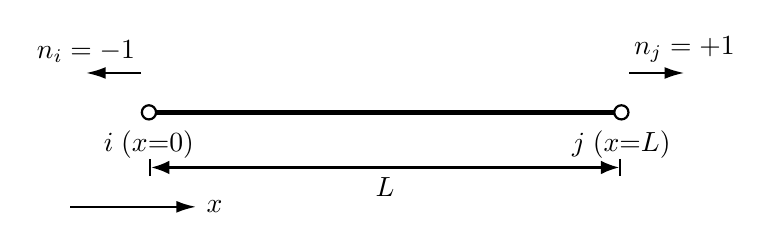
\begin{tikzpicture}[>={Latex[length=2.5mm, width=1.5mm]}]
    \coordinate (i) at (0,0);  \coordinate (j) at (6,0);
    \draw[line width=2pt] (i)--(j);
    \node[feNode, label=below:{$i\;(x{=}0)$}] at (i) {};
    \node[feNode, label=below:{$j\;(x{=}L)$}] at (j) {};
    \draw[->,thick] (-0.1,0.5)--(-0.8,0.5) node[above,pos=1]{$n_i=-1$};
    \draw[->,thick] (6.1,0.5)--(6.8,0.5) node[above,pos=1]{$n_j=+1$};
    \draw[dimLine] (0,-0.7)--(6,-0.7) node[midway,below]{$L$};
    \draw[->,thick] (-1.0,-1.2)--(0.6,-1.2) node[right]{$x$};
\end{tikzpicture}}
\caption{Element $(e)$: domain $[0,L]$ with outward unit normals.}
\label{fig:element}
\end{figure}

Let $P_1(e)$ be the space of affine functions on~$e$ spanned by the shape functions
\[
N_i(x)=1-\frac{x}{L},\qquad N_j(x)=\frac{x}{L},
\]
satisfying $N_\alpha(x_\beta)=\delta_{\alpha\beta}$ with $x_i:=0$, $x_j:=L$.  Any field $\phi_h\in P_1(e)$ is $\phi_h(x)=\sum_{\alpha}N_\alpha(x)\,\phi_\alpha$, $\phi_\alpha:=\phi_h(x_\alpha)$.

\begin{figure}[H]
\centering
\resizebox{0.55\textwidth}{!}{%
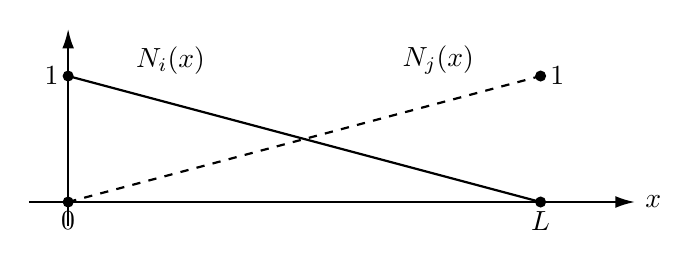
\begin{tikzpicture}[>={Latex[length=2.5mm, width=1.5mm]}]
    \draw[->,thick] (-0.5,0)--(7.2,0) node[right]{$x$};
    \draw[->,thick] (0,-0.3)--(0,2.2);
    \draw[thick,black] (0,1.6)--(6,0);
    \fill[black] (0,1.6) circle(2pt);  \fill[black] (6,0) circle(2pt);
    \node[black,left] at (0,1.6){$1$};
    \node[black,above] at (1.3,1.5){$N_i(x)$};
    \draw[thick,dashed,black] (0,0)--(6,1.6);
    \fill[black] (0,0) circle(2pt);  \fill[black] (6,1.6) circle(2pt);
    \node[black,right] at (6,1.6){$1$};
    \node[black,above] at (4.7,1.5){$N_j(x)$};
    \node[below] at (0,0){$0$};  \node[below] at (6,0){$L$};
\end{tikzpicture}}
\caption{Linear shape functions $N_i$ and $N_j$ on element $(e)$.}
\label{fig:shape}
\end{figure}

\subsection{Infinitesimal strain measure and constitutive laws}\label{sec:strain}

The one-dimensional infinitesimal (engineering) strain is defined as $\varepsilon(x):=du^{\mathrm{ax}}/dx$, where $u^{\mathrm{ax}}(x)$ is the axial displacement along the positive $x$-axis.  This is the linearized strain measure, valid for $|\varepsilon|\ll 1$, under which the strain--displacement relation is linear, the constitutive law $\sigma=E\varepsilon$ is appropriate, the stiffness matrix is constant, and equilibrium may be written on the undeformed configuration.  The constitutive laws for the three problems are:

\begin{table}[H]
\centering
\renewcommand{\arraystretch}{1.5}
\begin{tabular}{@{}lccc@{}}
\toprule
\textbf{Problem} & \textbf{Gradient} & \textbf{Constitutive law} & \textbf{Material const.}\\
\midrule
Truss (axial) & $\varepsilon=\dfrac{du^{\mathrm{ax}}}{dx}$ & $\sigma=E\,\varepsilon$ \;\;(Hooke) & $E>0$\\[6pt]
Cold conduction & $g=\dfrac{dT}{dx}$ & $q^c=k\,g$ \;\;(inv.\ Fourier) & $k>0$\\[6pt]
Electrical & $\mathcal{E}=-\dfrac{dV}{dx}$ & $J=\sigma_e\,\mathcal{E}$ \;\;(Ohm) & $\sigma_e>0$\\
\bottomrule
\end{tabular}
\caption{Constitutive relations for the three 1-D problems.}
\label{tab:const}
\end{table}

% ======================================================================
%  3. PROBLEM 1
% ======================================================================
\section{Problem 1: Truss Member Stiffness Matrix}

Let $u^{\mathrm{ax}}(x)\in P_1(e)$ be the axial displacement field.  Let the nodal degrees of freedom be the \emph{outward} components of the boundary displacement,
\[
u_\alpha:= u^{\mathrm{ax}}(x_\alpha)\,n_\alpha,\qquad \alpha\in\{i,j\},
\]
so that $u_i=-u^{\mathrm{ax}}(0)$ and $u_j=+u^{\mathrm{ax}}(L)$.  Let $\mathbf{u}:=\binom{u_i}{u_j}$.

\begin{figure}[H]
\centering
\resizebox{0.65\textwidth}{!}{%
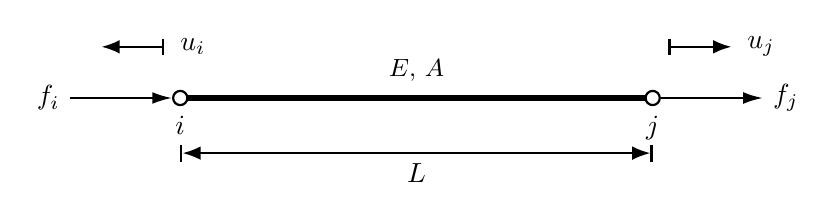
\begin{tikzpicture}[>={Latex[length=2.5mm, width=1.5mm]}]
    \coordinate (i) at (0,0);  \coordinate (j) at (6,0);
    \draw[line width=2pt] (i)--(j);
    \node[feNode, label=below:{$i$}] (NodeI) at (i) {};
    \node[feNode, label=below:{$j$}] (NodeJ) at (j) {};
    \draw[->,thick] (-1.4,0)--(NodeI) node[pos=0,left]{$f_i$};
    \draw[->,thick] (NodeJ)--(7.4,0) node[pos=1,right]{$f_j$};
    \draw[{Latex}-{Bar[width=2mm]},thick] (-1.0,0.65)--(-0.2,0.65) node[pos=1,right=2pt]{$u_i$};
    \draw[{Bar[width=2mm]}-{Latex},thick] (6.2,0.65)--(7.0,0.65) node[pos=1,right=2pt]{$u_j$};
    \draw[dimLine] (0,-0.7)--(6,-0.7) node[midway,below]{$L$};
    \node at (3,0.35) {\small $E,\,A$};
\end{tikzpicture}}
\caption{Truss element: DOFs positive outward.}
\label{fig:truss}
\end{figure}

The affine reconstruction consistent with $u^{\mathrm{ax}}(0)=-u_i$ and $u^{\mathrm{ax}}(L)=+u_j$ reads $u^{\mathrm{ax}}_h(x)=-N_i(x)\,u_i+N_j(x)\,u_j$.  The infinitesimal axial strain follows as
\[
\varepsilon(x)=\frac{du^{\mathrm{ax}}_h}{dx}
=\frac{d}{dx}\!\Bigl[-\!\bigl(1-\tfrac{x}{L}\bigr)\,u_i+\tfrac{x}{L}\,u_j\Bigr]
=\frac{u_i+u_j}{L},
\]
constant on $(e)$.  Let the constitutive law be $\sigma=E\,\varepsilon$ (Hooke) and the axial force $\mathcal{N}=A\,\sigma$, with $E>0$, $A>0$ constant.  Then $\sigma=\frac{E}{L}(u_i+u_j)$ and $\mathcal{N}=\frac{EA}{L}(u_i+u_j)$.

Let the stored elastic energy be $\mathcal{W}(\mathbf{u})=\frac{1}{2}\int_0^L EA\,\varepsilon^2\,dx=\frac{1}{2}\,\frac{EA}{L}\,(u_i+u_j)^2$.  Let $(f_i,f_j)$ be the energetic conjugates of $(u_i,u_j)$, i.e.\ $f_\alpha=\partial\mathcal{W}/\partial u_\alpha$.  Then
\[
f_i=\frac{EA}{L}(u_i+u_j),\qquad f_j=\frac{EA}{L}(u_i+u_j).
\]
Let $\mathbf{f}:=\binom{f_i}{f_j}$.  The element law $\mathbf{f}=K^{(e)}\,\mathbf{u}$ is therefore
\[
\boxed{
\begin{pmatrix} f_i\\[2pt] f_j\end{pmatrix}
=\frac{EA}{L}
\begin{pmatrix} 1 & 1\\[2pt] 1 & 1\end{pmatrix}
\begin{pmatrix} u_i\\[2pt] u_j\end{pmatrix}.
}
\]
Column~$\beta$ of $K^{(e)}$ is the force vector when $u_\beta=1$, $u_\gamma=0$ ($\gamma\neq\beta$):

\begin{figure}[H]
\centering
\resizebox{\textwidth}{!}{%
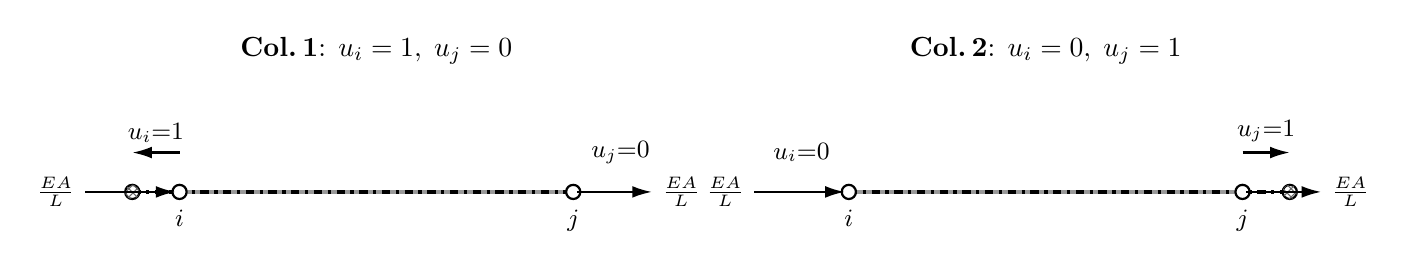
\begin{tikzpicture}[>={Latex[length=2.5mm, width=1.5mm]}]
    % --- Column 1 ---
    \begin{scope}[xshift=0cm]
        \node[anchor=south] at (2.5,1.5) {\textbf{Col.\,1}: $u_i=1,\;u_j=0$};
        \coordinate (i) at (0,0); \coordinate (j) at (5,0);
        \draw[line width=1.2pt,black!40] (i)--(j);
        \draw[line width=1.2pt,dash dot,black] (-0.6,0)--(5,0);
        \node[feNode] at (i){}; \node[feNode] at (j){};
        \node[feNode,fill=white,draw=black,postaction={pattern=crosshatch,pattern color=black!60}] at (-0.6,0){};
        \node[below] at (0,-0.1){\small $i$}; \node[below] at (5,-0.1){\small $j$};
        \draw[->,thick,black] (0,0.5)--(-0.6,0.5) node[midway,above]{\small $u_i{=}1$};
        \node[black] at (5.6,0.5){\small $u_j{=}0$};
        \draw[->,thick,black] (-1.2,0)--(-0.05,0) node[pos=0,left]{\small $\frac{EA}{L}$};
        \draw[->,thick,black] (5.05,0)--(6.0,0) node[pos=1,right]{\small $\frac{EA}{L}$};
    \end{scope}
    % --- Column 2 ---
    \begin{scope}[xshift=8.5cm]
        \node[anchor=south] at (2.5,1.5) {\textbf{Col.\,2}: $u_i=0,\;u_j=1$};
        \coordinate (i) at (0,0); \coordinate (j) at (5,0);
        \draw[line width=1.2pt,black!40] (i)--(j);
        \draw[line width=1.2pt,dash dot,black] (0,0)--(5.6,0);
        \node[feNode] at (i){}; \node[feNode] at (j){};
        \node[feNode,fill=white,draw=black,postaction={pattern=crosshatch,pattern color=black!60}] at (5.6,0){};
        \node[below] at (0,-0.1){\small $i$}; \node[below] at (5,-0.1){\small $j$};
        \node[black] at (-0.6,0.5){\small $u_i{=}0$};
        \draw[->,thick,black] (5,0.5)--(5.6,0.5) node[midway,above]{\small $u_j{=}1$};
        \draw[->,thick,black] (-1.2,0)--(-0.05,0) node[pos=0,left]{\small $\frac{EA}{L}$};
        \draw[->,thick,black] (5.05,0)--(6.0,0) node[pos=1,right]{\small $\frac{EA}{L}$};
    \end{scope}
\end{tikzpicture}}
\caption{Superposition: unit displacement states $\to$ columns of $K^{(e)}$.}
\label{fig:truss_super}
\end{figure}

$K^{(e)}$ is symmetric ($K^{(e)}_{\alpha\beta}=K^{(e)}_{\beta\alpha}$, Maxwell--Betti reciprocity) and positive semi-definite since $\mathbf{u}^{\!T}K^{(e)}\mathbf{u}=\frac{EA}{L}(u_i+u_j)^2\geq 0$ for all~$\mathbf{u}$.  It has $\mathrm{rank}(K^{(e)})=1$ and $\dim\ker(K^{(e)})=1$.  A rigid translation $u^{\mathrm{ax}}(x)\equiv c$ gives $u_i=-c$, $u_j=+c$, hence $\mathbf{u}_{\mathrm{rigid}}\propto\binom{-1}{+1}$; the nullspace verification is in \cref{sec:validation}.

% ======================================================================
%  4. PROBLEM 2
% ======================================================================
\section{Problem 2: ``Cold'' Conduction Matrix}

Let $T(x)\in P_1(e)$ be the temperature field with nodal values $T_i:=T(0)$, $T_j:=T(L)$, and let $\mathbf{T}:=\binom{T_i}{T_j}$.  The affine approximation and its gradient are
\[
T_h(x)=N_i(x)\,T_i+N_j(x)\,T_j,\qquad
\frac{dT_h}{dx}=\frac{T_j-T_i}{L}.
\]
Let the ``cold flux per area'' be defined by $q^c(x)=k\,dT_h/dx$, $k>0$; this is the sign-reversed Fourier law ($q^c=-q^h$), encoding ``cold flows from low to high temperature.''

\begin{figure}[H]
\centering
\resizebox{0.65\textwidth}{!}{%
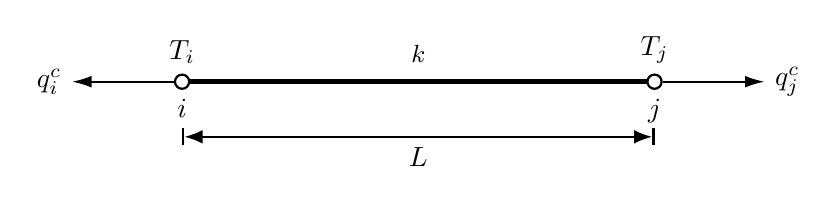
\begin{tikzpicture}[>={Latex[length=2.5mm, width=1.5mm]}]
    \coordinate (i) at (0,0);  \coordinate (j) at (6,0);
    \draw[line width=2pt] (i)--(j);
    \node[feNode, label=below:{$i$}, label=above:{$T_i$}] (NodeI) at (i) {};
    \node[feNode, label=below:{$j$}, label=above:{$T_j$}] (NodeJ) at (j) {};
    \draw[->,thick] (NodeI)--(-1.4,0) node[pos=1,left]{$q_i^c$};
    \draw[->,thick] (NodeJ)--(7.4,0) node[pos=1,right]{$q_j^c$};
    \draw[dimLine] (0,-0.7)--(6,-0.7) node[midway,below]{$L$};
    \node at (3,0.35) {\small $k$};
\end{tikzpicture}}
\caption{Cold conduction element: $q^c_\alpha>0$ outward.}
\label{fig:cold}
\end{figure}

Let the outward nodal cold fluxes per area be $q^c_\alpha:= q^c(x_\alpha)\,n_\alpha$, so $q^c_\alpha>0$ means directed out of the element.  Since $q^c=k(T_j-T_i)/L$ is constant on $(e)$,
\[
q_i^c=q^c\!\cdot\!(-1)=\frac{k}{L}(T_i-T_j),\qquad
q_j^c=q^c\!\cdot\!(+1)=\frac{k}{L}(T_j-T_i).
\]
Let $\mathbf{q}^c:=\binom{q^c_i}{q^c_j}$.  The element cold conduction law $\mathbf{q}^c=K^{(c)}\mathbf{T}$ is
\[
\boxed{
\begin{pmatrix} q_i^c\\[2pt] q_j^c\end{pmatrix}
=\frac{k}{L}
\begin{pmatrix} 1 & -1\\[2pt] -1 & 1\end{pmatrix}
\begin{pmatrix} T_i\\[2pt] T_j\end{pmatrix}.
}
\]
Let $A$ denote the cross-sectional area; the total cold rates are $\mathbf{Q}^c=A\,\mathbf{q}^c=\frac{kA}{L}\bigl(\begin{smallmatrix}1&-1\\-1&1\end{smallmatrix}\bigr)\mathbf{T}$.  The columns of $K^{(c)}$ arise from unit temperature states:

\begin{figure}[H]
\centering
\resizebox{\textwidth}{!}{%
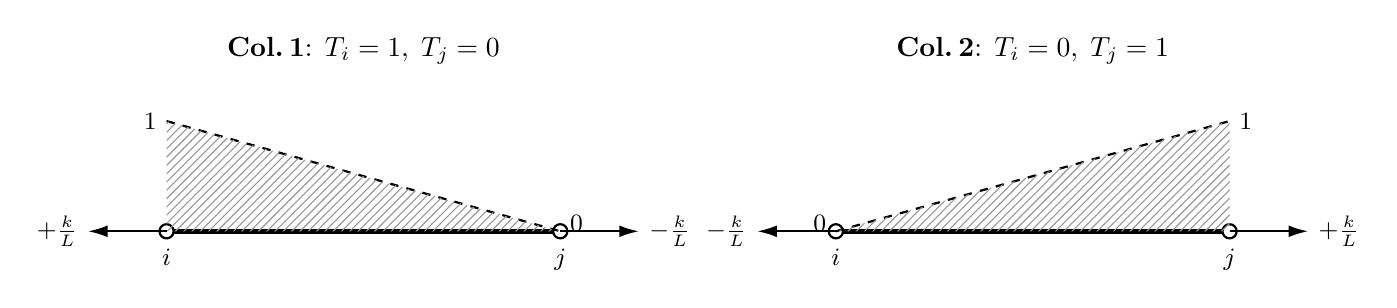
\begin{tikzpicture}[>={Latex[length=2.5mm, width=1.5mm]}]
    % --- Column 1 ---
    \begin{scope}[xshift=0cm]
        \node[anchor=south] at (2.5,2.0) {\textbf{Col.\,1}: $T_i=1,\;T_j=0$};
        \coordinate (i) at (0,0); \coordinate (j) at (5,0);
        \draw[line width=2pt] (i)--(j);
        \node[feNode] at (i){}; \node[feNode] at (j){};
        \node[below] at (0,-0.1){\small $i$}; \node[below] at (5,-0.1){\small $j$};
        \draw[thick,dashed,black] (0,1.4)--(5,0.0);
        \fill[pattern=north east lines, pattern color=black!40] (0,0)--(0,1.4)--(5,0)--cycle;
        \node[left,black] at (0,1.4){\small $1$};
        \node[right,black] at (5,0.1){\small $0$};
        \draw[->,thick] (0,0)--(-1.0,0) node[left]{\small $+\frac{k}{L}$};
        \draw[->,thick] (5,0)--(6.0,0) node[right]{\small $-\frac{k}{L}$};
    \end{scope}
    % --- Column 2 ---
    \begin{scope}[xshift=8.5cm]
        \node[anchor=south] at (2.5,2.0) {\textbf{Col.\,2}: $T_i=0,\;T_j=1$};
        \coordinate (i) at (0,0); \coordinate (j) at (5,0);
        \draw[line width=2pt] (i)--(j);
        \node[feNode] at (i){}; \node[feNode] at (j){};
        \node[below] at (0,-0.1){\small $i$}; \node[below] at (5,-0.1){\small $j$};
        \draw[thick,dashed,black] (0,0.0)--(5,1.4);
        \fill[pattern=north east lines, pattern color=black!40] (0,0)--(5,0)--(5,1.4)--cycle;
        \node[left,black] at (0,0.1){\small $0$};
        \node[right,black] at (5,1.4){\small $1$};
        \draw[->,thick] (0,0)--(-1.0,0) node[left]{\small $-\frac{k}{L}$};
        \draw[->,thick] (5,0)--(6.0,0) node[right]{\small $+\frac{k}{L}$};
    \end{scope}
\end{tikzpicture}}
\caption{Superposition: unit temperature states $\to$ columns of $K^{(c)}$.}
\label{fig:cold_super}
\end{figure}

$K^{(c)}$ is symmetric and positive semi-definite: $\mathbf{T}^{\!T}K^{(c)}\mathbf{T}=\frac{k}{L}(T_i-T_j)^2\geq 0$.  It has $\mathrm{rank}(K^{(c)})=1$.  A uniform temperature $T_i=T_j$ gives $dT_h/dx=0$, $\mathbf{q}^c=\mathbf{0}$, so $\binom{1}{1}\in\ker K^{(c)}$; the explicit check is in \cref{sec:validation}.

% ======================================================================
%  5. PROBLEM 3
% ======================================================================
\section{Problem 3: Resistive Wire Current Conduction Matrix}

Let $V(x)\in P_1(e)$ be the electric potential with nodal values $V_i:=V(0)$, $V_j:=V(L)$, and let $\mathbf{V}:=\binom{V_i}{V_j}$.  Then $V_h(x)=N_i(x)\,V_i+N_j(x)\,V_j$ and $dV_h/dx=(V_j-V_i)/L$.  Let the electric field be $\mathcal{E}(x)=-dV_h/dx$ and the current density obey Ohm's law $J(x)=\sigma_e\,\mathcal{E}(x)$, $\sigma_e>0$, so that
\[
J(x)=-\sigma_e\,\frac{V_j-V_i}{L}=\frac{\sigma_e}{L}(V_i-V_j),
\]
constant on $(e)$.

\begin{figure}[H]
\centering
\resizebox{0.65\textwidth}{!}{%
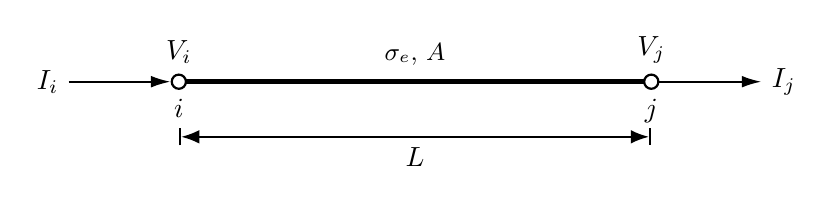
\begin{tikzpicture}[>={Latex[length=2.5mm, width=1.5mm]}]
    \coordinate (i) at (0,0);  \coordinate (j) at (6,0);
    \draw[line width=2pt] (i)--(j);
    \node[feNode, label=below:{$i$}, label=above:{$V_i$}] (NodeI) at (i) {};
    \node[feNode, label=below:{$j$}, label=above:{$V_j$}] (NodeJ) at (j) {};
    \draw[->,thick] (-1.4,0)--(NodeI) node[pos=0,left]{$I_i$};
    \draw[->,thick] (NodeJ)--(7.4,0) node[pos=1,right]{$I_j$};
    \draw[dimLine] (0,-0.7)--(6,-0.7) node[midway,below]{$L$};
    \node at (3,0.35) {\small $\sigma_e,\,A$};
\end{tikzpicture}}
\caption{Resistive wire element: $I_i$ into node~$i$, $I_j$ out of node~$j$.}
\label{fig:resist}
\end{figure}

Let the nodal currents be the outward normal fluxes of $J$ over area~$A$: $I_\alpha:= A\,J(x_\alpha)\,n_\alpha$.  Using $n_i=-1$, $n_j=+1$,
\begin{align}
I_i&= A\,J\cdot(-1)=\frac{\sigma_e A}{L}(-V_i+V_j),\\[4pt]
I_j&= A\,J\cdot(+1)=\frac{\sigma_e A}{L}(V_i-V_j).
\end{align}
Let $\mathbf{I}:=\binom{I_i}{I_j}$.  The element current--potential relation $\mathbf{I}=K^{(R)}\mathbf{V}$ is
\[
\boxed{
\begin{pmatrix} I_i\\[2pt] I_j\end{pmatrix}
=\frac{\sigma_e A}{L}
\begin{pmatrix} -1 & 1\\[2pt] 1 & -1\end{pmatrix}
\begin{pmatrix} V_i\\[2pt] V_j\end{pmatrix}.
}
\]
Let $R:=L/(\sigma_e A)$ be the resistance and $G:=R^{-1}=\sigma_e A/L$ the conductance; the same relation is $\mathbf{I}=G\!\begin{psmallmatrix}-1&1\\1&-1\end{psmallmatrix}\!\mathbf{V}$.  The columns of $K^{(R)}$ arise from unit potential states:

\begin{figure}[H]
\centering
\resizebox{\textwidth}{!}{%
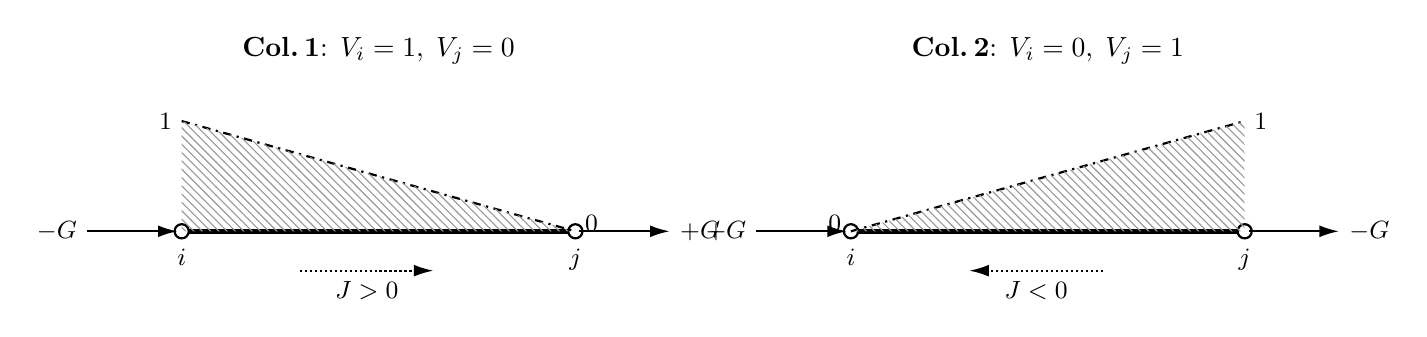
\begin{tikzpicture}[>={Latex[length=2.5mm, width=1.5mm]}]
    % --- Column 1 ---
    \begin{scope}[xshift=0cm]
        \node[anchor=south] at (2.5,2.0) {\textbf{Col.\,1}: $V_i=1,\;V_j=0$};
        \coordinate (i) at (0,0); \coordinate (j) at (5,0);
        \draw[line width=2pt] (i)--(j);
        \node[feNode] at (i){}; \node[feNode] at (j){};
        \node[below] at (0,-0.1){\small $i$}; \node[below] at (5,-0.1){\small $j$};
        \draw[thick,dash dot,black] (0,1.4)--(5,0.0);
        \fill[pattern=north west lines, pattern color=black!40] (0,0)--(0,1.4)--(5,0)--cycle;
        \node[left,black] at (0,1.4){\small $1$};
        \node[right,black] at (5,0.1){\small $0$};
        \draw[->,thick] (-1.2,0)--(-0.05,0) node[pos=0,left]{\small $-G$};
        \draw[->,thick] (5.05,0)--(6.2,0) node[pos=1,right]{\small $+G$};
        \draw[->,thick,densely dotted,black] (1.5,-0.5)--(3.2,-0.5) node[midway,below]{\small $J>0$};
    \end{scope}
    % --- Column 2 ---
    \begin{scope}[xshift=8.5cm]
        \node[anchor=south] at (2.5,2.0) {\textbf{Col.\,2}: $V_i=0,\;V_j=1$};
        \coordinate (i) at (0,0); \coordinate (j) at (5,0);
        \draw[line width=2pt] (i)--(j);
        \node[feNode] at (i){}; \node[feNode] at (j){};
        \node[below] at (0,-0.1){\small $i$}; \node[below] at (5,-0.1){\small $j$};
        \draw[thick,dash dot,black] (0,0.0)--(5,1.4);
        \fill[pattern=north west lines, pattern color=black!40] (0,0)--(5,0)--(5,1.4)--cycle;
        \node[left,black] at (0,0.1){\small $0$};
        \node[right,black] at (5,1.4){\small $1$};
        \draw[->,thick] (-1.2,0)--(-0.05,0) node[pos=0,left]{\small $+G$};
        \draw[->,thick] (5.05,0)--(6.2,0) node[pos=1,right]{\small $-G$};
        \draw[->,thick,densely dotted,black] (3.2,-0.5)--(1.5,-0.5) node[midway,below]{\small $J<0$};
    \end{scope}
\end{tikzpicture}}
\caption{Superposition: unit potential states $\to$ columns of $K^{(R)}$.}
\label{fig:resist_super}
\end{figure}

$K^{(R)}$ is symmetric and \emph{negative} semi-definite: $\mathbf{V}^{\!T}K^{(R)}\mathbf{V}=-G(V_i-V_j)^2\leq 0$; the negative sign arises because the homework's current convention (into~$i$, out of~$j$) is not a purely outward convention.  Under the standard convention $\mathbf{I}^{\mathrm{in}}:=-\mathbf{I}$ one recovers the positive semi-definite conductance matrix $\mathbf{I}^{\mathrm{in}}=G\bigl(\begin{smallmatrix}1&-1\\-1&1\end{smallmatrix}\bigr)\mathbf{V}$.  The matrix has $\mathrm{rank}(K^{(R)})=1$, and a uniform potential $V_i=V_j$ gives $\mathcal{E}=0$, $J=0$, confirming $\binom{1}{1}\in\ker K^{(R)}$; see \cref{sec:validation}.

% ======================================================================
%  6. SUMMARY
% ======================================================================
\section{Summary}

\begin{table}[H]
    \centering
    \renewcommand{\arraystretch}{1.8}
    \begin{tabular}{|l|c|c|c|}
        \hline
        \textbf{Quantity} & \textbf{Pr.\,1 (Truss)} & \textbf{Pr.\,2 (Cold Cond.)} & \textbf{Pr.\,3 (Electrical)} \\
        \hline
        Primary variable & $u$ (displacement) & $T$ (temperature) & $V$ (potential) \\
        \hline
        Gradient & $\varepsilon = \dfrac{du}{dx}$ & $g = \dfrac{dT}{dx}$ & $\mathcal{E} = -\dfrac{dV}{dx}$ \\
        \hline
        Constitutive law & $\sigma = E\varepsilon$ & $q^c = k g$ & $J = \sigma_e \mathcal{E}$ \\
        \hline
        Material property & $E$ (Young's mod.) & $k$ (therm.\ cond.) & $\sigma_e$ (elec.\ cond.) \\
        \hline
        Flux / Force & $f$ (force) & $q^c$ (cold flux) & $I$ (current) \\
        \hline
        Element matrix & $\dfrac{EA}{L} \begin{pmatrix} 1 & 1 \\ 1 & 1 \end{pmatrix}$ & $\dfrac{k}{L} \begin{pmatrix} 1 & -1 \\ -1 & 1 \end{pmatrix}$ & $\dfrac{\sigma_e A}{L} \begin{pmatrix} -1 & 1 \\ 1 & -1 \end{pmatrix}$ \\
        \hline
        Nullspace vector & $\begin{pmatrix} -1 \\ +1 \end{pmatrix}$ & $\begin{pmatrix} 1 \\ 1 \end{pmatrix}$ & $\begin{pmatrix} 1 \\ 1 \end{pmatrix}$ \\
        \hline
        Physical meaning & rigid translation & uniform temp. & uniform potential \\
        \hline
    \end{tabular}
    \caption{Cross-domain analogy for the three 1D finite element problems.}
    \label{tab:summary}
\end{table}

\vspace{0.3cm}

\noindent \textbf{Key observation:} The three matrices differ only in sign pattern, a direct consequence of the \textit{different sign conventions} for the degrees of freedom at boundary nodes:

\textbf{Problem 1:} Outward displacement DOF $\Rightarrow$ sign flip at node $i$ $\Rightarrow$ all-positive matrix.
\textbf{Problem 2:} Standard nodal values, outward flux $\Rightarrow$ classical symmetric positive semidefinite conduction matrix.
\textbf{Problem 3:} Into-$i$/out-of-$j$ current convention $\Rightarrow$ negative semidefinite; flip to ``into-element'' convention recovers the standard form.

% ======================================================================
%  7. VALIDATION
% ======================================================================
\section{Validation: Nullspace (Zero-Gradient Mode) Checks}\label{sec:validation}

Each element matrix must annihilate the DOF vector corresponding to the trivial (zero-gradient) state of the respective field.  The three verifications are as follows.

\medskip
\noindent\textbf{Problem 1 --- Rigid-body translation.}\quad A rigid translation $u^{\mathrm{ax}}(x)\equiv c$ gives $u_i = n_i\,c = -c$ and $u_j = n_j\,c = +c$, hence $\mathbf{u}_{\mathrm{rigid}}\propto\binom{-1}{+1}$ and $\varepsilon = (u_i+u_j)/L = 0$.  Substituting into the element law:
\[
K^{(e)}\!\begin{pmatrix}-1\\+1\end{pmatrix}
=\frac{EA}{L}\!\begin{pmatrix}1&1\\1&1\end{pmatrix}\!\begin{pmatrix}-1\\+1\end{pmatrix}
=\frac{EA}{L}\!\begin{pmatrix}-1+1\\-1+1\end{pmatrix}
=\begin{pmatrix}0\\0\end{pmatrix}.\quad\checkmark
\]

\medskip
\noindent\textbf{Problem 2 --- Uniform temperature.}\quad A uniform temperature $T_i = T_j$ gives $dT_h/dx = (T_j - T_i)/L = 0$, hence $q^c = 0$ and $\mathbf{q}^c = \mathbf{0}$.  The nullspace vector is $\binom{1}{1}$:
\[
K^{(c)}\!\begin{pmatrix}1\\1\end{pmatrix}
=\frac{k}{L}\!\begin{pmatrix}1&-1\\-1&1\end{pmatrix}\!\begin{pmatrix}1\\1\end{pmatrix}
=\frac{k}{L}\!\begin{pmatrix}1-1\\-1+1\end{pmatrix}
=\begin{pmatrix}0\\0\end{pmatrix}.\quad\checkmark
\]

\medskip
\noindent\textbf{Problem 3 --- Uniform potential.}\quad A uniform potential $V_i = V_j$ gives $dV_h/dx = 0$, $\mathcal{E} = 0$, $J = 0$, and no current flows.  The nullspace vector is $\binom{1}{1}$:
\[
K^{(R)}\!\begin{pmatrix}1\\1\end{pmatrix}
=\frac{\sigma_e A}{L}\!\begin{pmatrix}-1&1\\1&-1\end{pmatrix}\!\begin{pmatrix}1\\1\end{pmatrix}
=\frac{\sigma_e A}{L}\!\begin{pmatrix}-1+1\\1-1\end{pmatrix}
=\begin{pmatrix}0\\0\end{pmatrix}.\quad\checkmark
\]

\medskip
All three matrices are confirmed to be rank-1, symmetric, and to possess a physically meaningful one-dimensional nullspace corresponding to the zero-gradient mode of the respective field.

% ======================================================================
%  8. DISCUSSION
% ======================================================================
\section{Discussion: Sign Convention and Its Implication on the Kernel}

The choice of positive direction for the nodal degrees of freedom is not merely a labelling convention; it directly determines the sign pattern of the element stiffness matrix and, consequently, the algebraic form of its kernel vector.  This section discusses this relationship for all three problems.

In Problem~1 the DOFs are defined as the \emph{outward} displacement components $u_\alpha=u^{\mathrm{ax}}(x_\alpha)\,n_\alpha$.  Because $n_i=-1$, the DOF at node~$i$ has the opposite sign of the physical displacement.  A rigid translation $u^{\mathrm{ax}}\equiv c$ therefore maps to $u_i=-c$, $u_j=+c$, giving the kernel vector $\binom{-1}{+1}$.  This sign flip at node~$i$ is also the reason why $K^{(e)}$ has all-positive entries: both columns produce force in the same direction.

In Problem~2 the DOFs are simply the nodal temperatures $T_i$, $T_j$, with no sign reversal at either node.  A uniform temperature $T_i=T_j=c$ gives the kernel vector $\binom{1}{1}$.  The matrix $K^{(c)}$ has the classical pattern $\bigl(\begin{smallmatrix}+1&-1\\-1&+1\end{smallmatrix}\bigr)$, positive semi-definite, because the DOF convention and the flux convention are both standard outward.

In Problem~3 the DOFs are again plain nodal values $V_i$, $V_j$, so a uniform potential gives $\binom{1}{1}\in\ker K^{(R)}$, just like Problem~2.  However, the homework specifies current \emph{into} node~$i$ and \emph{out of} node~$j$, which is not a purely outward convention.  This mixed sign in the current direction introduces a global sign flip: $K^{(R)}=-G\bigl(\begin{smallmatrix}1&-1\\-1&1\end{smallmatrix}\bigr)$, making it negative semi-definite.  If one redefines $\mathbf{I}^{\mathrm{in}}:=-\mathbf{I}$ (all currents into the element), the standard positive semi-definite form is recovered.

\cref{tab:convention} collects the sign convention, the resulting matrix definiteness, and the kernel vector for each problem.

\begin{table}[H]
    \centering
    \renewcommand{\arraystretch}{1.6}
    \begin{tabular}{|l|c|c|c|}
        \hline
        & \textbf{Pr.\,1 (Truss)} & \textbf{Pr.\,2 (Cold Cond.)} & \textbf{Pr.\,3 (Electrical)} \\
        \hline
        DOF definition & $u_\alpha = u^{\mathrm{ax}} n_\alpha$ & $T_\alpha = T(x_\alpha)$ & $V_\alpha = V(x_\alpha)$ \\
        \hline
        Sign convention & outward disp. & nodal value & nodal value \\
        \hline
        Flux / force conv. & outward & outward & into-$i$, out-of-$j$ \\
        \hline
        Figure & \cref{fig:truss} & \cref{fig:cold} & \cref{fig:resist} \\
        \hline
        Element matrix sign & all $+$ & $\bigl(\begin{smallmatrix}+&-\\-&+\end{smallmatrix}\bigr)$ & $\bigl(\begin{smallmatrix}-&+\\+&-\end{smallmatrix}\bigr)$ \\
        \hline
        Definiteness & pos.\ semi-def. & pos.\ semi-def. & neg.\ semi-def. \\
        \hline
        Kernel vector & $\begin{pmatrix}-1\\+1\end{pmatrix}$ & $\begin{pmatrix}1\\1\end{pmatrix}$ & $\begin{pmatrix}1\\1\end{pmatrix}$ \\
        \hline
        Zero-gradient mode & rigid translation & uniform temp. & uniform potential \\
        \hline
    \end{tabular}
    \caption{Sign convention, matrix definiteness, and kernel vector for each problem.}
    \label{tab:convention}
\end{table}

The key insight is that all three kernels encode the same physics: a spatially constant field produces zero gradient and therefore zero internal force or flux.  The algebraic form of the kernel vector, however, depends on how the DOFs relate to the physical field.  When the DOF includes a sign reversal (as in Problem~1), the kernel vector inherits that reversal.

% ======================================================================
%  9. CONCLUSION
% ======================================================================
\section{Conclusion}

All three matrices were derived step by step.  They are all rank-1 and symmetric.  Each has a nullspace with a clear physical meaning.  The sign patterns come from the DOF conventions.  The results were checked in \cref{sec:validation}.

\end{document}
